\documentclass{standalone}
\usepackage{tikz}
\usetikzlibrary{patterns, positioning}
\usepackage[sfdefault]{ClearSans} %% option 'sfdefault' activates Clear Sans as the default text font
\usepackage[T1]{fontenc}

\begin{document}
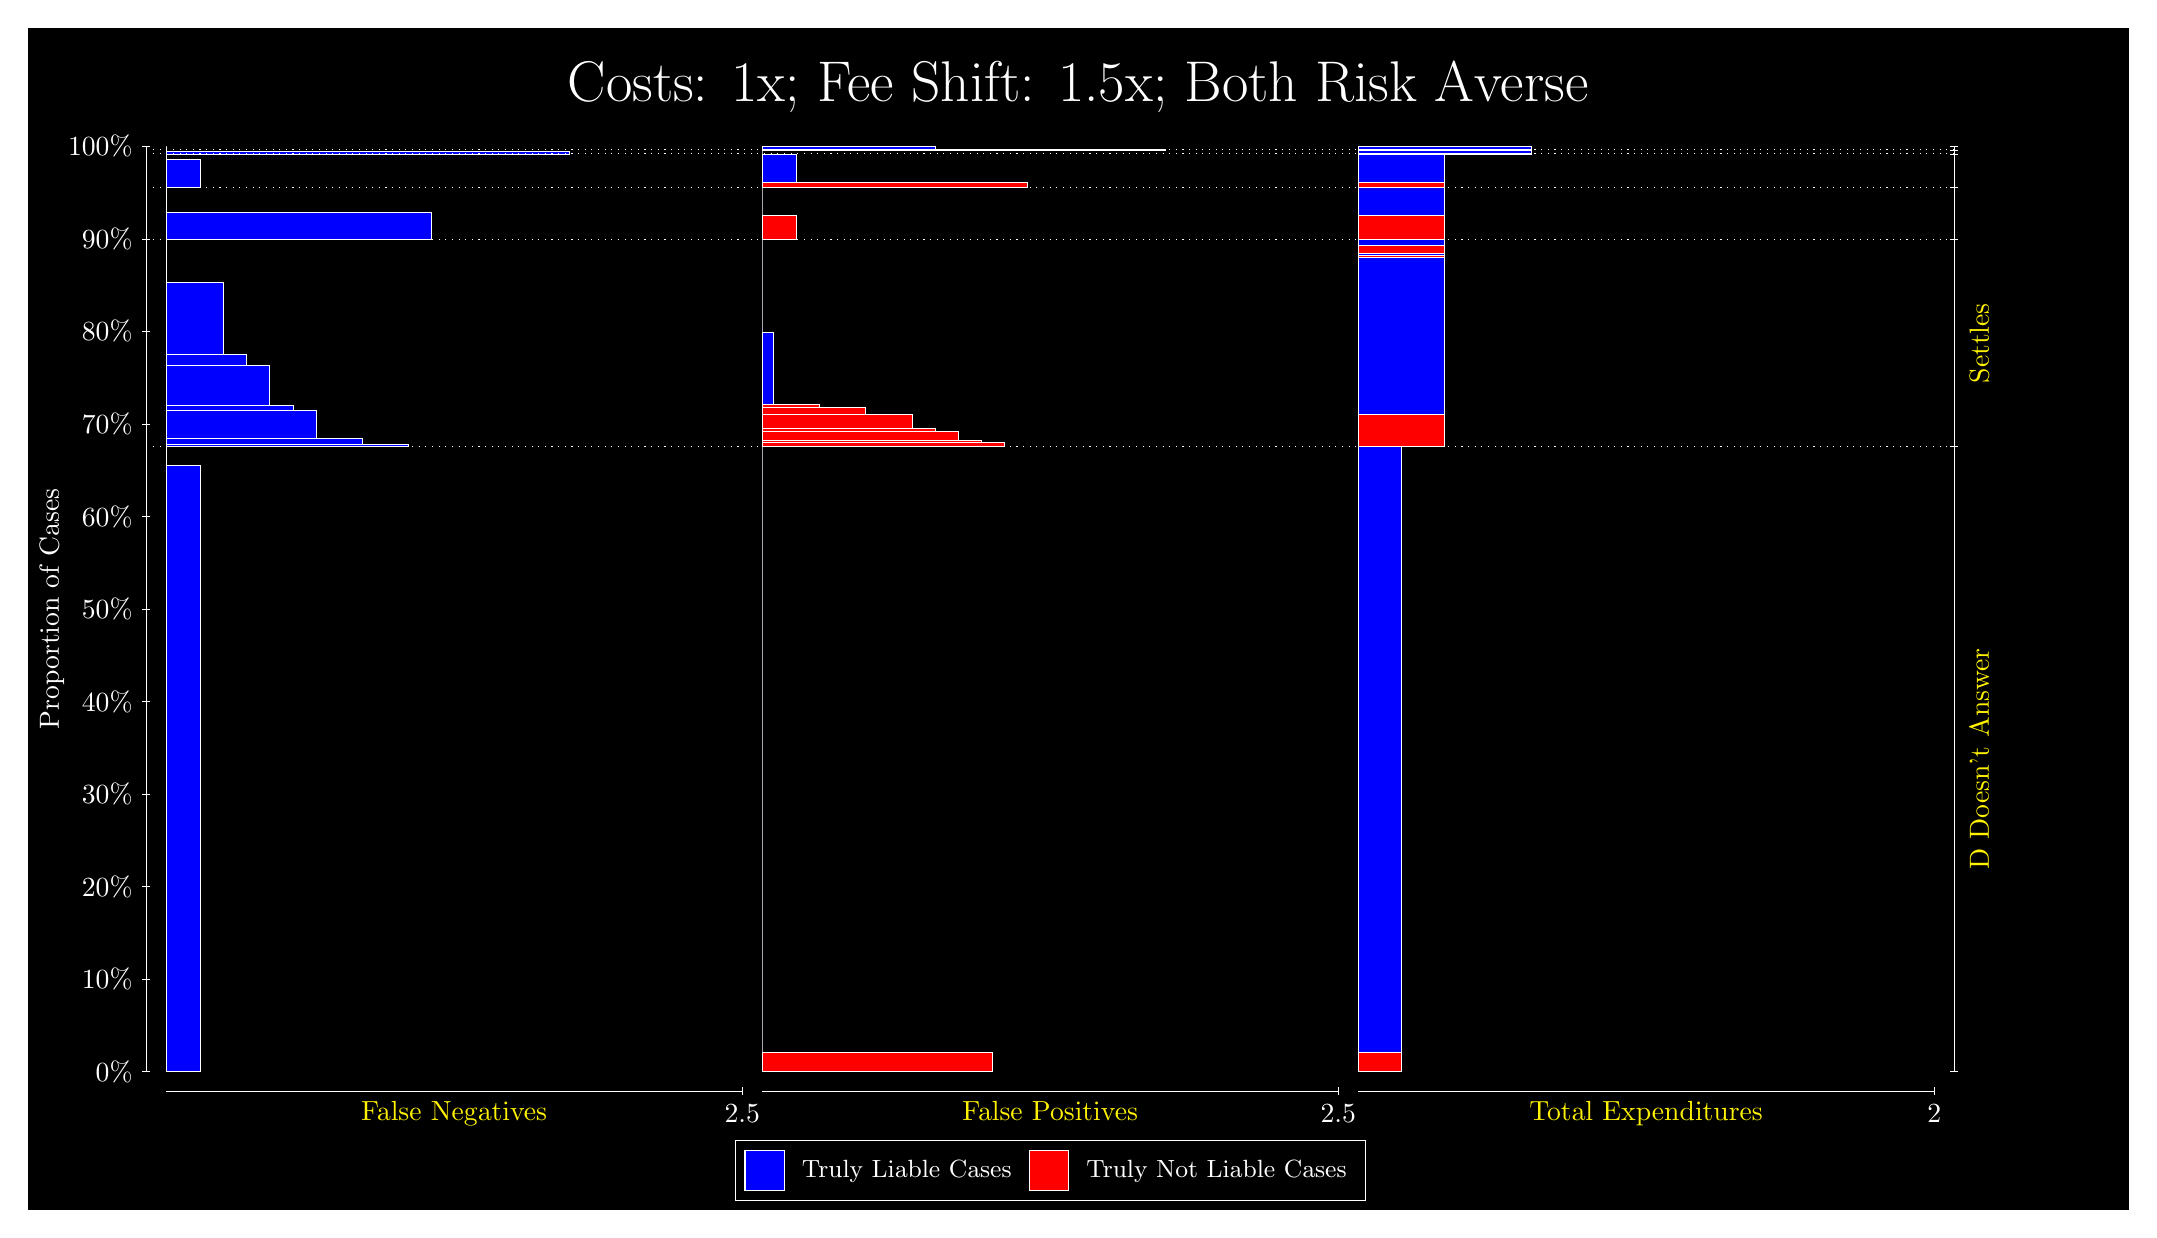
\begin{tikzpicture}
\draw[fill=black] (0,0) rectangle (26.667,15);
\draw[text=white] (0,13.5) rectangle (26.667,15) node[midway] {\huge Costs: 1x; Fee Shift: 1.5x; Both Risk Averse};
\draw[white, very thin] (1.5,1.75) -- (1.5,13.5);
\node[rotate=90, text=white, anchor=center] at (0.3, 7.625) {Proportion of Cases};
\draw[white, very thin] (1.45,1.75) -- (1.55,1.75);
\node[text=white, anchor=east] at (1.45, 1.75) {0\%};
\draw[white, very thin] (1.45,2.925) -- (1.55,2.925);
\node[text=white, anchor=east] at (1.45, 2.925) {10\%};
\draw[white, very thin] (1.45,4.1) -- (1.55,4.1);
\node[text=white, anchor=east] at (1.45, 4.1) {20\%};
\draw[white, very thin] (1.45,5.275) -- (1.55,5.275);
\node[text=white, anchor=east] at (1.45, 5.275) {30\%};
\draw[white, very thin] (1.45,6.45) -- (1.55,6.45);
\node[text=white, anchor=east] at (1.45, 6.45) {40\%};
\draw[white, very thin] (1.45,7.625) -- (1.55,7.625);
\node[text=white, anchor=east] at (1.45, 7.625) {50\%};
\draw[white, very thin] (1.45,8.8) -- (1.55,8.8);
\node[text=white, anchor=east] at (1.45, 8.8) {60\%};
\draw[white, very thin] (1.45,9.975) -- (1.55,9.975);
\node[text=white, anchor=east] at (1.45, 9.975) {70\%};
\draw[white, very thin] (1.45,11.15) -- (1.55,11.15);
\node[text=white, anchor=east] at (1.45, 11.15) {80\%};
\draw[white, very thin] (1.45,12.325) -- (1.55,12.325);
\node[text=white, anchor=east] at (1.45, 12.325) {90\%};
\draw[white, very thin] (1.45,13.5) -- (1.55,13.5);
\node[text=white, anchor=east] at (1.45, 13.5) {100\%};

\draw[white, very thin] (24.457,1.75) -- (24.457,13.5);
\draw[white, very thin] (24.407,1.75) -- (24.507,1.75);
\node[anchor=west] at (24.407, 1.75) {};
\draw[white, very thin] (24.407,9.6867) -- (24.507,9.6867);
\node[anchor=west] at (24.407, 9.6867) {};
\draw[white, very thin] (24.407,12.314) -- (24.507,12.314);
\node[anchor=west] at (24.407, 12.314) {};
\draw[white, very thin] (24.407,12.98) -- (24.507,12.98);
\node[anchor=west] at (24.407, 12.98) {};
\draw[white, very thin] (24.407,13.405) -- (24.507,13.405);
\node[anchor=west] at (24.407, 13.405) {};
\draw[white, very thin] (24.407,13.454) -- (24.507,13.454);
\node[anchor=west] at (24.407, 13.454) {};
\draw[white, very thin] (24.407,13.5) -- (24.507,13.5);
\node[anchor=west] at (24.407, 13.5) {};

\draw[white, very thin, fill=blue] (1.75,1.75) rectangle (2.1891,9.4457);
\draw[white, very thin, fill=red] (1.75,9.4457) rectangle (1.75,9.6867);
\draw[white, very thin, fill=blue] (1.75,9.6867) rectangle (4.8239,9.7125);
\draw[white, very thin, fill=blue] (1.75,9.7125) rectangle (4.2384,9.7877);
\draw[white, very thin, fill=blue] (1.75,9.7877) rectangle (3.9457,9.7897);
\draw[white, very thin, fill=blue] (1.75,9.7897) rectangle (3.6529,10.148);
\draw[white, very thin, fill=blue] (1.75,10.148) rectangle (3.3602,10.207);
\draw[white, very thin, fill=blue] (1.75,10.207) rectangle (3.0674,10.717);
\draw[white, very thin, fill=blue] (1.75,10.717) rectangle (2.7746,10.862);
\draw[white, very thin, fill=blue] (1.75,10.862) rectangle (2.4819,11.776);
\draw[white, very thin, fill=red] (1.75,11.776) rectangle (1.75,12.314);
\draw[white, very thin, fill=blue] (1.75,12.314) rectangle (5.1167,12.668);
\draw[white, very thin, fill=red] (1.75,12.668) rectangle (1.75,12.98);
\draw[white, very thin, fill=blue] (1.75,12.98) rectangle (2.1891,13.337);
\draw[white, very thin, fill=red] (1.75,13.337) rectangle (1.75,13.405);
\draw[white, very thin, fill=blue] (1.75,13.405) rectangle (6.8732,13.441);
\draw[white, very thin, fill=red] (1.75,13.441) rectangle (1.75,13.454);
\draw[white, very thin, fill=red] (1.75,13.454) rectangle (1.75,13.458);
\draw[white, very thin, fill=blue] (1.75,13.458) rectangle (1.75,13.5);
\draw[white, very thin, fill=red] (9.3189,1.75) rectangle (12.246,1.991);
\draw[white, very thin, fill=blue] (9.3189,1.991) rectangle (9.3189,9.6867);
\draw[white, very thin, fill=red] (9.3189,9.6867) rectangle (12.393,9.7439);
\draw[white, very thin, fill=red] (9.3189,9.7439) rectangle (12.1,9.7708);
\draw[white, very thin, fill=red] (9.3189,9.7708) rectangle (11.807,9.8763);
\draw[white, very thin, fill=red] (9.3189,9.8763) rectangle (11.515,9.9199);
\draw[white, very thin, fill=red] (9.3189,9.9199) rectangle (11.222,10.101);
\draw[white, very thin, fill=red] (9.3189,10.101) rectangle (10.929,10.102);
\draw[white, very thin, fill=red] (9.3189,10.102) rectangle (10.636,10.19);
\draw[white, very thin, fill=red] (9.3189,10.19) rectangle (10.051,10.224);
\draw[white, very thin, fill=blue] (9.3189,10.224) rectangle (9.4652,11.138);
\draw[white, very thin, fill=blue] (9.3189,11.138) rectangle (9.3189,12.314);
\draw[white, very thin, fill=red] (9.3189,12.314) rectangle (9.758,12.626);
\draw[white, very thin, fill=blue] (9.3189,12.626) rectangle (9.3189,12.98);
\draw[white, very thin, fill=red] (9.3189,12.98) rectangle (12.686,13.048);
\draw[white, very thin, fill=blue] (9.3189,13.048) rectangle (9.758,13.405);
\draw[white, very thin, fill=red] (9.3189,13.405) rectangle (9.3189,13.418);
\draw[white, very thin, fill=blue] (9.3189,13.418) rectangle (9.3189,13.454);
\draw[white, very thin, fill=red] (9.3189,13.454) rectangle (14.442,13.458);
\draw[white, very thin, fill=blue] (9.3189,13.458) rectangle (11.515,13.5);
\draw[white, very thin, fill=red] (16.888,1.75) rectangle (17.437,1.991);
\draw[white, very thin, fill=blue] (16.888,1.991) rectangle (17.437,9.6867);
\draw[white, very thin, fill=red] (16.888,9.6867) rectangle (17.986,10.101);
\draw[white, very thin, fill=blue] (16.888,10.101) rectangle (17.986,12.087);
\draw[white, very thin, fill=red] (16.888,12.087) rectangle (17.986,12.121);
\draw[white, very thin, fill=blue] (16.888,12.121) rectangle (17.986,12.147);
\draw[white, very thin, fill=red] (16.888,12.147) rectangle (17.986,12.237);
\draw[white, very thin, fill=blue] (16.888,12.237) rectangle (17.986,12.314);
\draw[white, very thin, fill=red] (16.888,12.314) rectangle (17.986,12.626);
\draw[white, very thin, fill=blue] (16.888,12.626) rectangle (17.986,12.98);
\draw[white, very thin, fill=red] (16.888,12.98) rectangle (17.986,13.048);
\draw[white, very thin, fill=blue] (16.888,13.048) rectangle (17.986,13.405);
\draw[white, very thin, fill=red] (16.888,13.405) rectangle (19.083,13.418);
\draw[white, very thin, fill=blue] (16.888,13.418) rectangle (19.083,13.454);
\draw[white, very thin, fill=red] (16.888,13.454) rectangle (19.083,13.458);
\draw[white, very thin, fill=blue] (16.888,13.458) rectangle (19.083,13.5);
\draw[white, dotted] (1.5,9.6867) -- (24.457,9.6867);
\draw[white, dotted] (1.5,12.314) -- (24.457,12.314);
\draw[white, dotted] (1.5,12.98) -- (24.457,12.98);
\draw[white, dotted] (1.5,13.405) -- (24.457,13.405);
\draw[white, dotted] (1.5,13.454) -- (24.457,13.454);
\draw[white, very thin] (1.75,1.5) -- (9.0689,1.5);
\node[text=yellow, anchor=north] at (5.4094, 1.5) {False Negatives};
\draw[white, very thin] (9.0689,1.45) -- (9.0689,1.55);
\node[text=white, anchor=north] at (9.0689, 1.45) {2.5};

\draw[white, very thin] (9.3189,1.5) -- (16.638,1.5);
\node[text=yellow, anchor=north] at (12.978, 1.5) {False Positives};
\draw[white, very thin] (16.638,1.45) -- (16.638,1.55);
\node[text=white, anchor=north] at (16.638, 1.45) {2.5};

\draw[white, very thin] (16.888,1.5) -- (24.207,1.5);
\node[text=yellow, anchor=north] at (20.547, 1.5) {Total Expenditures};
\draw[white, very thin] (24.207,1.45) -- (24.207,1.55);
\node[text=white, anchor=north] at (24.207, 1.45) {2};

\node[text=yellow, centered, rotate=90] at (24.777, 5.7184) {D Doesn't Answer};
\node[text=yellow, centered, rotate=90] at (24.777, 11) {Settles};





\draw (12.978300999999998,1.5) node[draw=none] (baseCoordinate) {};
\begin{scope}[align=center]
        \matrix[scale=0.5, draw=white, below=0.5cm of baseCoordinate, nodes={draw}, column sep=0.1cm]{
            \node[rectangle, draw, minimum width=0.5cm, minimum height=0.5cm, fill=blue] {}; &
            \node[draw=none, font=\small, text=white] (B) {Truly Liable Cases}; &
            \node[rectangle, draw, minimum width=0.5cm, minimum height=0.5cm, fill=red] {}; &
            \node[draw=none, font=\small, text=white] (B) {Truly Not Liable Cases}; \\
            };
\end{scope}

\end{tikzpicture}
\end{document}